\documentclass[/home/jesse/Analysis/FemtoAnalysis/AnalysisNotes/AnalysisNoteJBuxton.tex]{subfiles}

\renewcommand{\NonFlatBgdLamKch}{_NonFlatBgdCrctnLamK0LinearLamKchPolynomial}
\renewcommand{\NonFlatBgdLamKs}{_NonFlatBgdCrctnLamK0LinearLamKchPolynomial}

\renewcommand{\ResNum}{_10Res}
\renewcommand{\PrimMaxDecay}{_PrimMaxDecay4fm}

\renewcommand{\SaveNameModLamKch}{\MomRes\NonFlatBgdLamKch\ResNum\PrimMaxDecay\ResMethod\ParamFixAndShareLamKch}
\renewcommand{\SaveNameModLamKs}{\MomRes\NonFlatBgdLamKs\ResNum\PrimMaxDecay\ResMethod\ParamFixAndShareLamKch}

\begin{document}

\subsection{10 Residual Contributors Included in Fit}
\label{App_ResultsLamK_10Res}

This section presents fit results for which 10 residual contributors were assumed.
These contributors include those shared by the three contributor case (App. \ref{App_ResultsLamK_3Res}), ($\Sigma^{0}\mathrm{K}$, $\Xi^{0}\mathrm{K}$, $\Xi^{-}\mathrm{K}$) $\rightarrow \Lambda\mathrm{K}$, and additionally the contributors ($\Sigma^{* (+,-,0)}\mathrm{K}^{*0}$, $\Lambda\mathrm{K}^{*0}$, $\Sigma^{0}\mathrm{K}^{*0}$, $\Xi^{0}\mathrm{K}^{*0}$, $\Xi^{-}\mathrm{K}^{*0}$) $\rightarrow \Lambda\mathrm{K}$.
As stated at the beginning of App. \ref{App_Results}, most of the $\Sigma^{*}$ and $\mathrm{K}^{*}$ resonances will have decayed before kinetic freeze-out, and therefore it is best to treat $\Lambda$ and $\mathrm{K}$ particles originating from these resonances as primary, i.e. only using three residual contributors.
However, it is still interesting to examine how these additional shorter lived sources affect our fit result, as presented below.
For a comparison of these results to the case of three residual contributors, see Fig. \ref{figApp:Comparisons_3v10vNo} in App. \ref{App_ResultsLamK_FitMethComp}

%%%%%%%%%%%%%%%%%%%%%%%%%%%%%%%%%%%%%%%%%%%%%%%%%%%%%%%%%%%%%%%%%%%%%%
\begin{figure}[h]
  \centering
  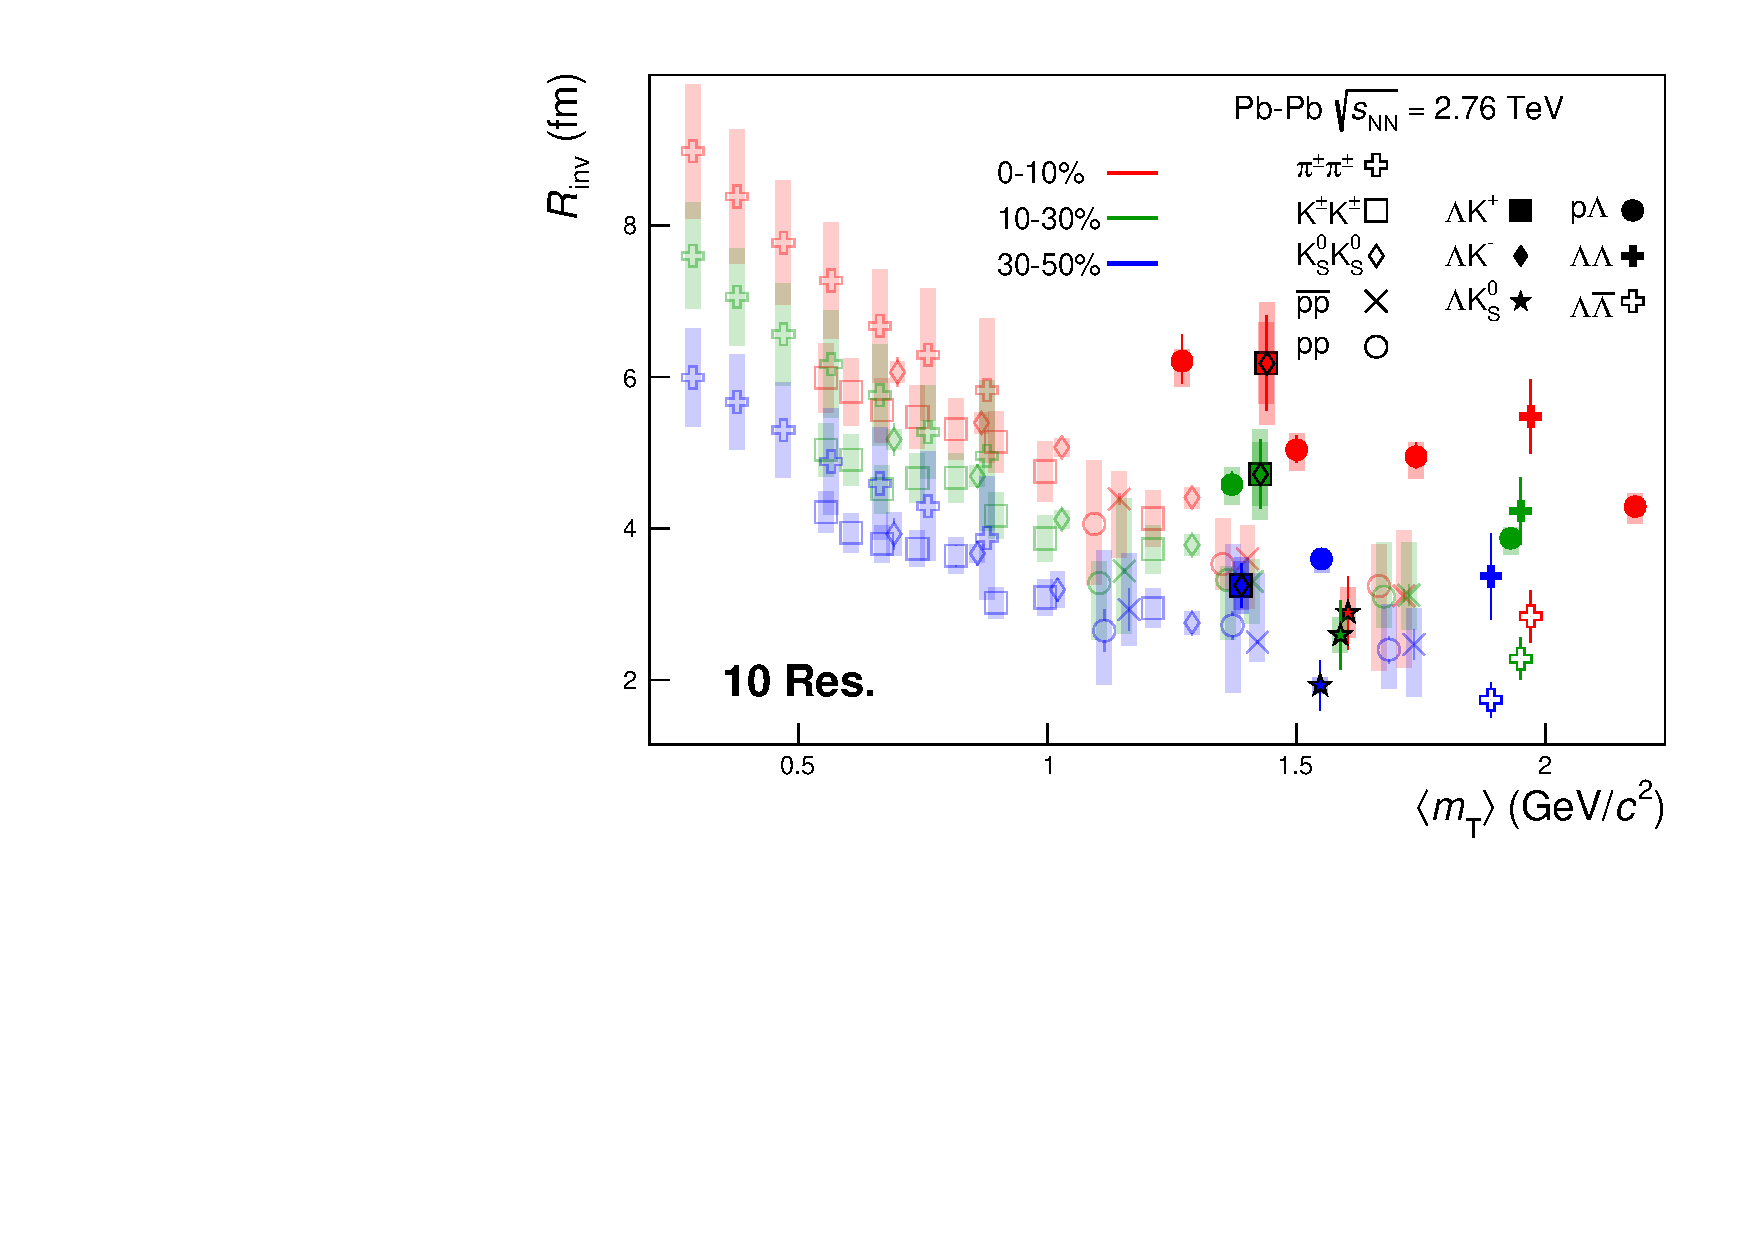
\includegraphics[width=0.80\textwidth]{\ResultsDirBaseLamKch\SaveNameModLamKch/Comparisons/mTscaling_MinvCalc_OutlinedPoints_OthersTransparent_wJaiAndHans_10Res.pdf}
  \caption[$m_{\mathrm{T}}$ scaling of radii: 10 residuals]
  {
  10 residual correlations in \LamK fits.  
  Extracted fit $R_{\mathrm{inv}}$ parameters as a function of pair transverse mass ($m_{\mathrm{T}}$) for various pair systems over several centralities. 
  The ALICE published data \cite{Adam:2015vja} are shown with transparent, open symbols.  
  The new \LamK results are shown with opaque, filled symbols.  
  The \mt value for the \LamK system is an average of those for the \LamKchP, \ALamKchM, and \LamKs systems.
  }
  \label{figApp:mTScalingOfRadii_10Res}
\end{figure}


\begin{figure}[h]
  \centering
  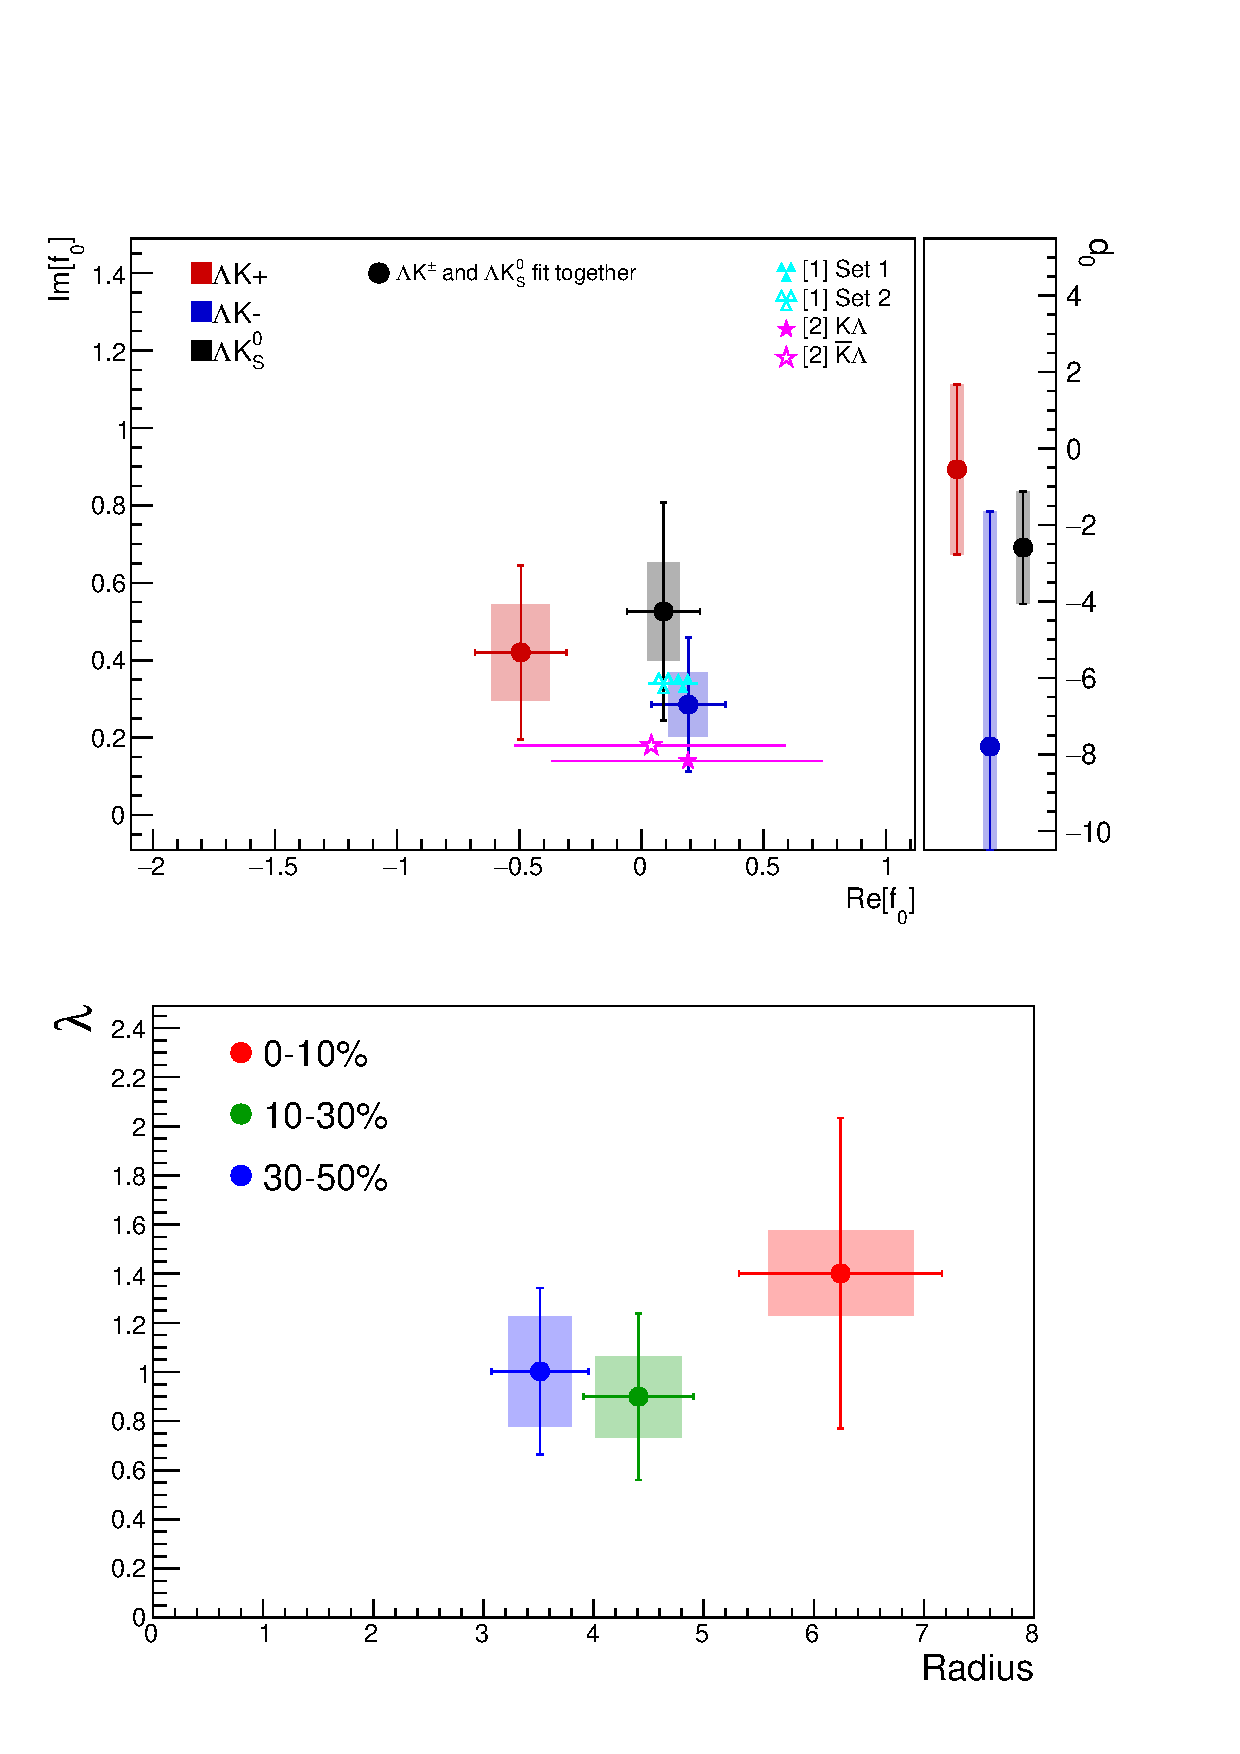
\includegraphics[width=0.65\textwidth]{\ResultsDirBaseLamKch\SaveNameModLamKch/Comparisons/FinalResults_Comp3An_Vertical.pdf}
  \caption[Extracted scattering parameters: 10 residuals]
  {
  Extracted fit parameters for the case of 10 residual contributors for all of our \LamK systems.  
  [Top]: $\Im f_{0}$ vs. $\Re f_{0}$, together with $d_{0}$ to the right.  
  [Bottom]: $\lambda$ vs. Radius for the 0-10\% (blue), 10-30\% (green), and 30-50\% (red) centrality bins.  
  In the fit, all \LamK systems share common radii.
  The color scheme used in the panel are to be consistent with those in Fig. \ref{figApp:mTScalingOfRadii_10Res}.
  The cyan ([A] = Ref. \cite{Liu:2006xja}) and magenta ([B] = Ref. \cite{Mai:2009ce}) points show theoretical predictions made using chiral perturbation theory.  
  }
  \label{figApp:ScattParams_10Res}
\end{figure}


%%%%%%%%%%%%%%%%%%%%%%%%%%%%%%%%%%%%%%%%%%%%%%%%%%%%%%%%%%%%%%%%%%%%%%
\begin{figure}[h]
  \centering
  \includegraphics[width=0.75\textwidth]{\ResultsDirBaseLamKch\SaveNameModLamKch/canKStarCfwFitsLamKchPwConj_0010_1030_3050UnZoomed\SaveNameModLamKch.pdf}
  \caption[\LamKchPALamKchM data with fits: 10 residuals]
  {
  Fit results, with 10 residual correlations included, for the \LamKchP and \ALamKchM data.
  The \LamKchP data is shown in the left column, the \ALamKchM in the right, and the rows differentiate the different centrality bins (0-10\% in the top, 10-30\% in the middle, and 30-50\% in the bottom).
  }
  \label{figApp:LamKchPwConjFits_10Res}
\end{figure}


\begin{figure}[h]
  \centering
  \includegraphics[width=0.75\textwidth]{\ResultsDirBaseLamKch\SaveNameModLamKch/Residuals\ResNum/LamKchP/canKStarCfwFitsAndResidualsLamKchPwConj_0010_1030_3050UnZoomed_ZoomResiduals\SaveNameModLamKch.pdf}
  \caption[\LamKchPALamKchM fit contribution from residuals: 10 residuals]
  {
  Fit results with the 10 residual contributions shown, for the \LamKchP and \ALamKchM data.
  The \LamKchP data is shown in the left column, the \ALamKchM in the right, and the rows differentiate the different centrality bins (0-10\% in the top, 10-30\% in the middle, and 30-50\% in the bottom).
  }
  \label{figApp:LamKchPwConjFitsAndResiduals_10Res}
\end{figure}





%%%%%%%%%%%%%%%%%%%%%%%%%%%%%%%%%%%%%%%%%%%%%%%%%%%%%%%%%%%%%%%%%%%%%%
\begin{figure}[h]
  \centering
  \includegraphics[width=0.75\textwidth]{\ResultsDirBaseLamKch\SaveNameModLamKch/canKStarCfwFitsLamKchMwConj_0010_1030_3050UnZoomed\SaveNameModLamKch.pdf}
  \caption[\LamKchMALamKchP data with fits: 10 residuals]
  {
  Fit results, with 10 residual correlations included, for the \LamKchM and \ALamKchP data.
  The \LamKchM data is shown in the left column, the \ALamKchP in the right, and the rows differentiate the different centrality bins (0-10\% in the top, 10-30\% in the middle, and 30-50\% in the bottom).
  }
  \label{figApp:LamKchMwConjFits_10Res}
\end{figure}


\begin{figure}[h]
  \centering
  \includegraphics[width=0.75\textwidth]{\ResultsDirBaseLamKch\SaveNameModLamKch/Residuals\ResNum/LamKchM/canKStarCfwFitsAndResidualsLamKchMwConj_0010_1030_3050UnZoomed_ZoomResiduals\SaveNameModLamKch.pdf}
  \caption[\LamKchMALamKchP fit contribution from residuals: 10 residuals]
  {
  Fit results with the 10 residual contributions shown, for the \LamKchM and \ALamKchP data.
  The \LamKchM data is shown in the left column, the \ALamKchP in the right, and the rows differentiate the different centrality bins (0-10\% in the top, 10-30\% in the middle, and 30-50\% in the bottom).
  }
  \label{figApp:LamKchMwConjFitsAndResiduals_10Res}
\end{figure}




%%%%%%%%%%%%%%%%%%%%%%%%%%%%%%%%%%%%%%%%%%%%%%%%%%%%%%%%%%%%%%%%%%%%%%
\begin{figure}[h]
  \centering
  \includegraphics[width=0.75\textwidth]{\ResultsDirBaseLamKs\SaveNameModLamKs/canKStarCfwFitsLamK0wConj_0010_1030_3050UnZoomed\SaveNameModLamKs.pdf}
  \caption[\LamALamKs data with fits: 10 residuals]
  {
  Fit results, with 10 residual correlations included, for the \LamKs and \ALamKs data.
  The \LamKs data is shown in the left column, the \ALamKs in the right, and the rows differentiate the different centrality bins (0-10\% in the top, 10-30\% in the middle, and 30-50\% in the bottom).
  }
  \label{figApp:LamKswConjFits_10Res}
\end{figure}


\begin{figure}[h]
  \centering
  \includegraphics[width=0.75\textwidth]{\ResultsDirBaseLamKs\SaveNameModLamKs/Residuals\ResNum/LamK0/canKStarCfwFitsAndResidualsLamK0wConj_0010_1030_3050UnZoomed_ZoomResiduals\SaveNameModLamKs.pdf}
  \caption[\LamKsALamKs fit contribution from residuals: 10 residuals]
  {
  Fit results with the 10 residual contributions shown, for the \LamKs and \ALamKs data.
  The \LamKs data is shown in the left column, the \ALamKs in the right, and the rows differentiate the different centrality bins (0-10\% in the top, 10-30\% in the middle, and 30-50\% in the bottom).
  }
  \label{figApp:LamKswConjFitsAndResiduals_10Res}
\end{figure}

\begin{comment}
%%%%%%%%%%%%%%%%%%%%%%%%%%%%%%%%%%%%%%%%     TABLES!!!!!     %%%%%%%%%%%%%%%%%%%%%%%%%%%%%%%%%%%%%%%%
%\pagestyle{empty}
\begin{landscape}

\subfile{\ResultsDirBaseLamKch\SaveNameModLamKch/Tables/ResultsTableTriple.tex}

\end{landscape}
%\pagestyle{plain}
%%%%%%%%%%%%%%%%%%%%%%%%%%%%%%%%%%%%%%%%%%%%%%%%%%%%%%%%%%%%%%%%%%%%%%%%%%%%%%%%%%%%%%%%%%%%%%%%%%%%%
\end{comment}

\clearpage

\end{document}